
%(BEGIN_QUESTION)
% Copyright 2007, Tony R. Kuphaldt, released under the Creative Commons Attribution License (v 1.0)
% This means you may do almost anything with this work of mine, so long as you give me proper credit

In this system a variable-frequency drive (VFD) sends AC electrical power to an induction motor to control the speed of that motor.  The VFD receives its ``command'' signal in the form of a 4-20 mA DC current sent from a programmable logic controller (PLC) with an analog output card, 4 mA representing a ``zero-speed'' signal (no power sent to the motor) and 20 mA representing a ``full speed'' signal (60 Hz power sent to the motor):

$$\includegraphics[width=15.5cm]{i02554x01.eps}$$

Unfortunately, though, there is something wrong with this system.  The pump does not run, regardless of what the operator commands using the touch-screen panel.  When you examine the VFD faceplate, you see a few LED indicators lit, but nothing either confirming or denying that power is reaching the motor.

Supposing the only test equipment available to you is a digital multimeter (DMM), what diagnostic tests could you perform to identify the location and nature of the system fault?

\vskip 20pt \vbox{\hrule \hbox{\strut \vrule{} {\bf Suggestions for Socratic discussion} \vrule} \hrule}

\begin{itemize}
\item{} Why might one opt to use a VFD to control a pump's speed, rather than just use a throttling valve to control how much fluid is discharged from a constant-speed pump?
\end{itemize}

\underbar{file i02554}
%(END_QUESTION)





%(BEGIN_ANSWER)


%(END_ANSWER)





%(BEGIN_NOTES)

The fact that there are lit LEDs on the VFD faceplate tells us the VFD has AC power supplied to it.  A good diagnostic test would be to use the multimeter to measure the 4-20 mA command signal at the VFD's terminals, to check and see if the VFD is being commanded to run the motor.  If not, then the problem is either in the 4-20 mA cable or somewhere in the PLC system.  If there is a non-stopped 4-20 mA signal present at the VFD terminals, then the problem may lie either with the VFD, the motor, or the power cables between the VFD and motor.

%INDEX% Basics, control loop troubleshooting: determining reason why VFD won't run
%INDEX% Final Control Elements: troubleshooting

%(END_NOTES)


